
\section{Unsupervised Analysis}\label{sec:unsupervised}

We apply PCA to reduce both feature representations to 2D and run k-means clustering on the training set.
We use $k=2$ for visualization (corresponding to the two insect orders) and $k=66$ to compute Normalized Mutual Information (NMI) against true species labels.
NMI ranges from 0 (no alignment) to 1 (perfect alignment).

For MFCC features, the first two principal components explain 31.1\% of variance and NMI~$= 0.58$.
For log-mel features, NMI~$= 0.587$, marginally higher than MFCC.
Both feature types show partial order-level separation: Cicadidae form a compact cluster while Orthoptera spread more widely.
The high NMI confirms that both feature types encode substantial species-discriminative information without supervision.

\begin{figure}[!t]
    \centering
    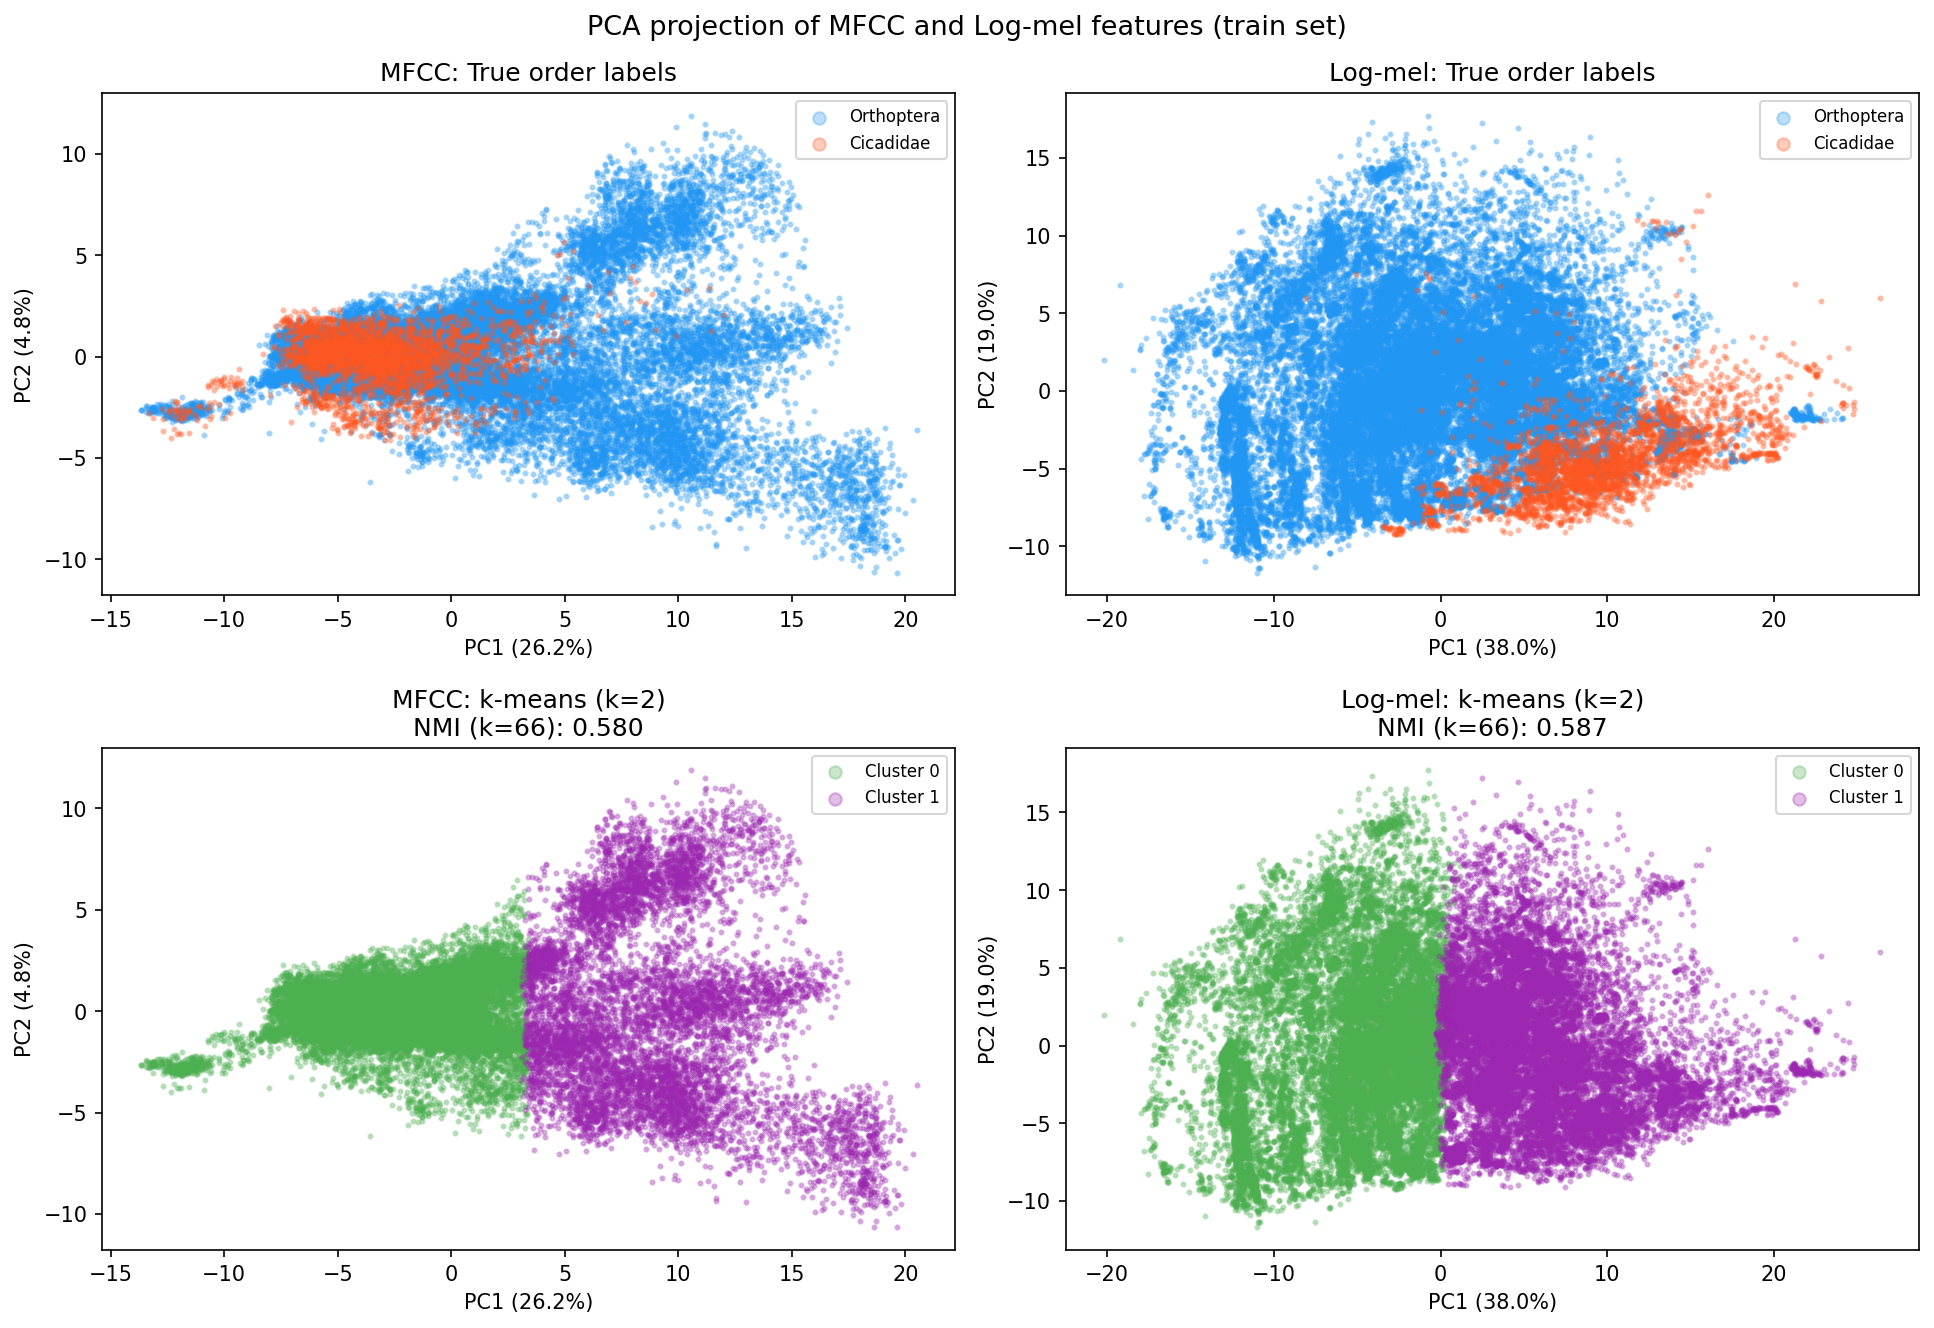
\includegraphics[width=\columnwidth]{images/pca_kmeans_both.png}
    \caption{PCA projection of MFCC (left) and log-mel (right) features on the training set. Top row: true order labels. Bottom row: k-means ($k=2$) cluster assignments. NMI scores ($k=66$) are shown in panel titles.}
    \label{fig:pca}
\end{figure}

\section{Classification Results}\label{sec:results}

Table~\ref{table:results} summarizes validation and test performance for all models.
SVM achieves the highest test accuracy (76.7\%) and macro-F1 (0.71).
Random Forest reaches 75.4\% accuracy and 0.64 macro-F1.
Both classical models outperform our replicated mel-CNN (60.4\%).
The CNN was trained without data augmentation; Fai\ss{} and Stowell~\cite{faiss2023adaptive} report 82\% (mel-5, with augmentation, median of 3 seeds).

\begin{table}[!t]
\caption{Classification performance on InsectSet66 (66 classes). Bold indicates best result per column among our models.}
\label{table:results}
\centering
\resizebox{\columnwidth}{!}{%
\begin{tabular}{llrrrr}
\toprule
\multirow{2}{*}{Model} & \multirow{2}{*}{Features} & \multicolumn{2}{c}{Validation} & \multicolumn{2}{c}{Test} \\
\cmidrule(lr){3-4} \cmidrule(lr){5-6}
 &  & Acc & Macro-F1 & Acc & Macro-F1 \\
\midrule
SVM (RBF)            & MFCC           & 0.744 & \textbf{0.633} & \textbf{0.767} & \textbf{0.711} \\
Random Forest        & MFCC           & \textbf{0.748} & 0.601 & 0.754 & 0.637 \\
Mel-CNN (replicated) & Log-mel        & ---   & ---   & 0.604 & 0.514 \\
Mel-CNN~\cite{faiss2023adaptive} & Log-mel + aug. & 0.81 & --- & 0.82 & 0.74 \\
\bottomrule
\end{tabular}}
\end{table}


Figures~\ref{fig:cm_svm} and~\ref{fig:cm_rf} show the test-set confusion matrices.
The diagonal is dominant, indicating most chunks are correctly classified.
Errors are concentrated among a few acoustically similar species, consistent with the dataset's class imbalance.

\begin{figure}[!t]
    \centering
    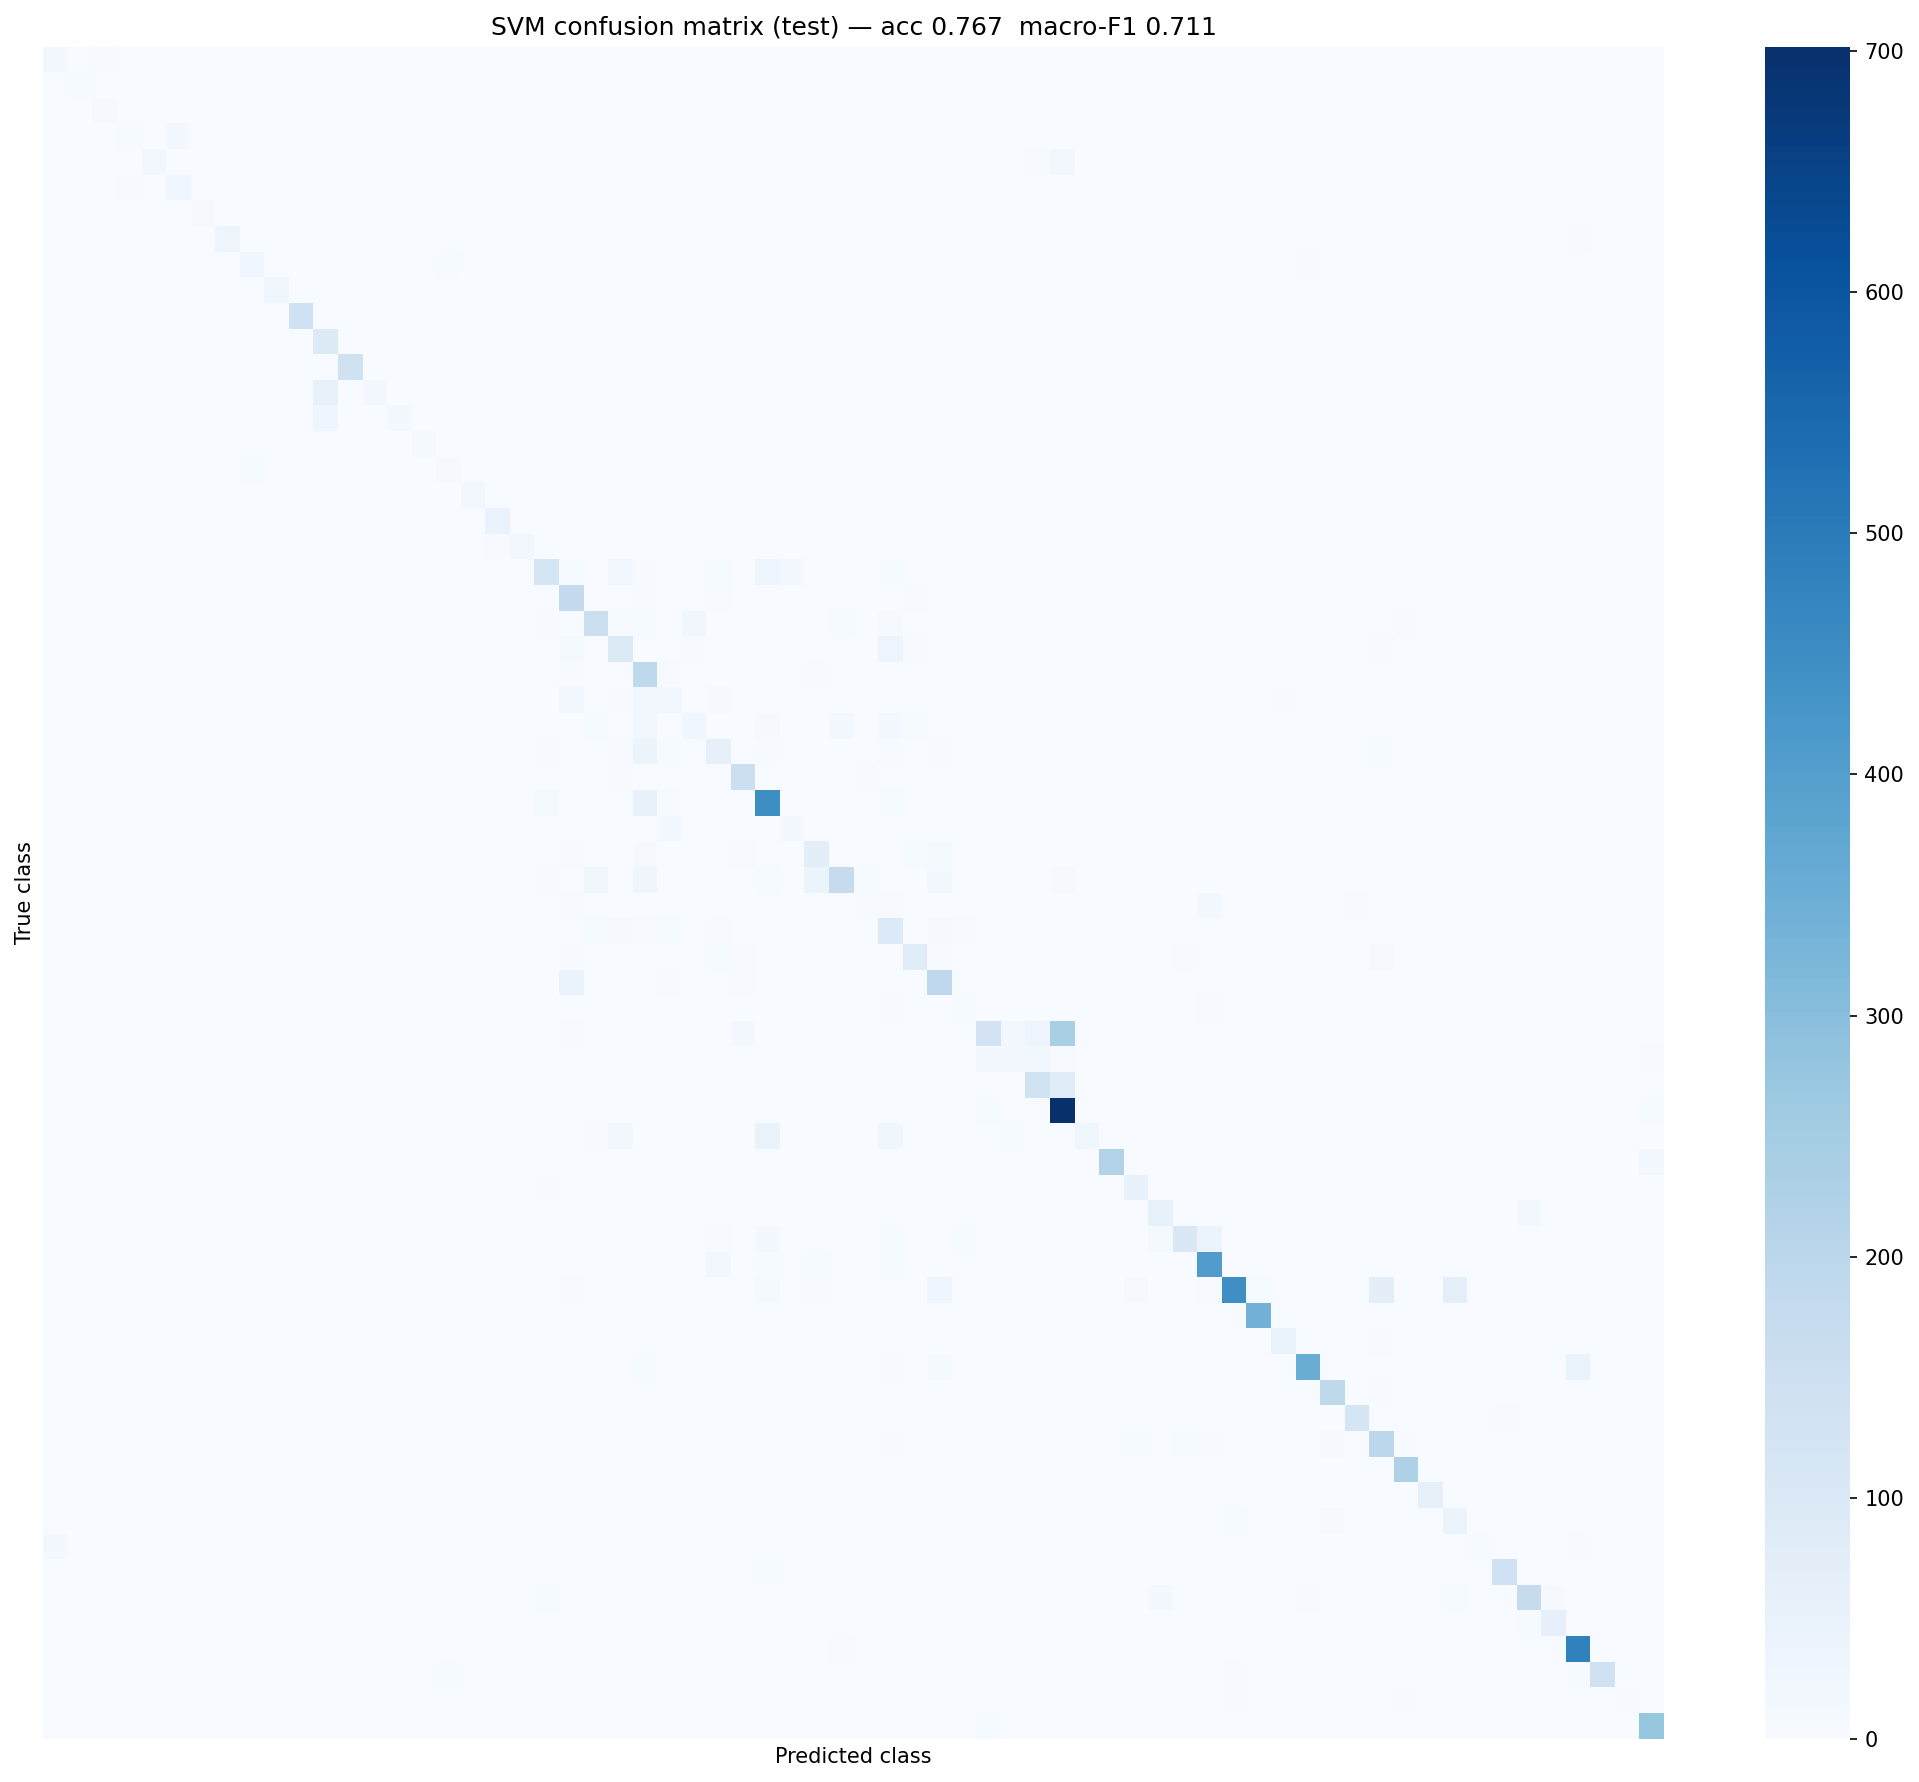
\includegraphics[width=\columnwidth]{images/confusion_matrix_svm.png}
    \caption{SVM confusion matrix on the test set (66 classes). Accuracy: 76.7\%, macro-F1: 0.71.}
    \label{fig:cm_svm}
\end{figure}

\begin{figure}[!t]
    \centering
    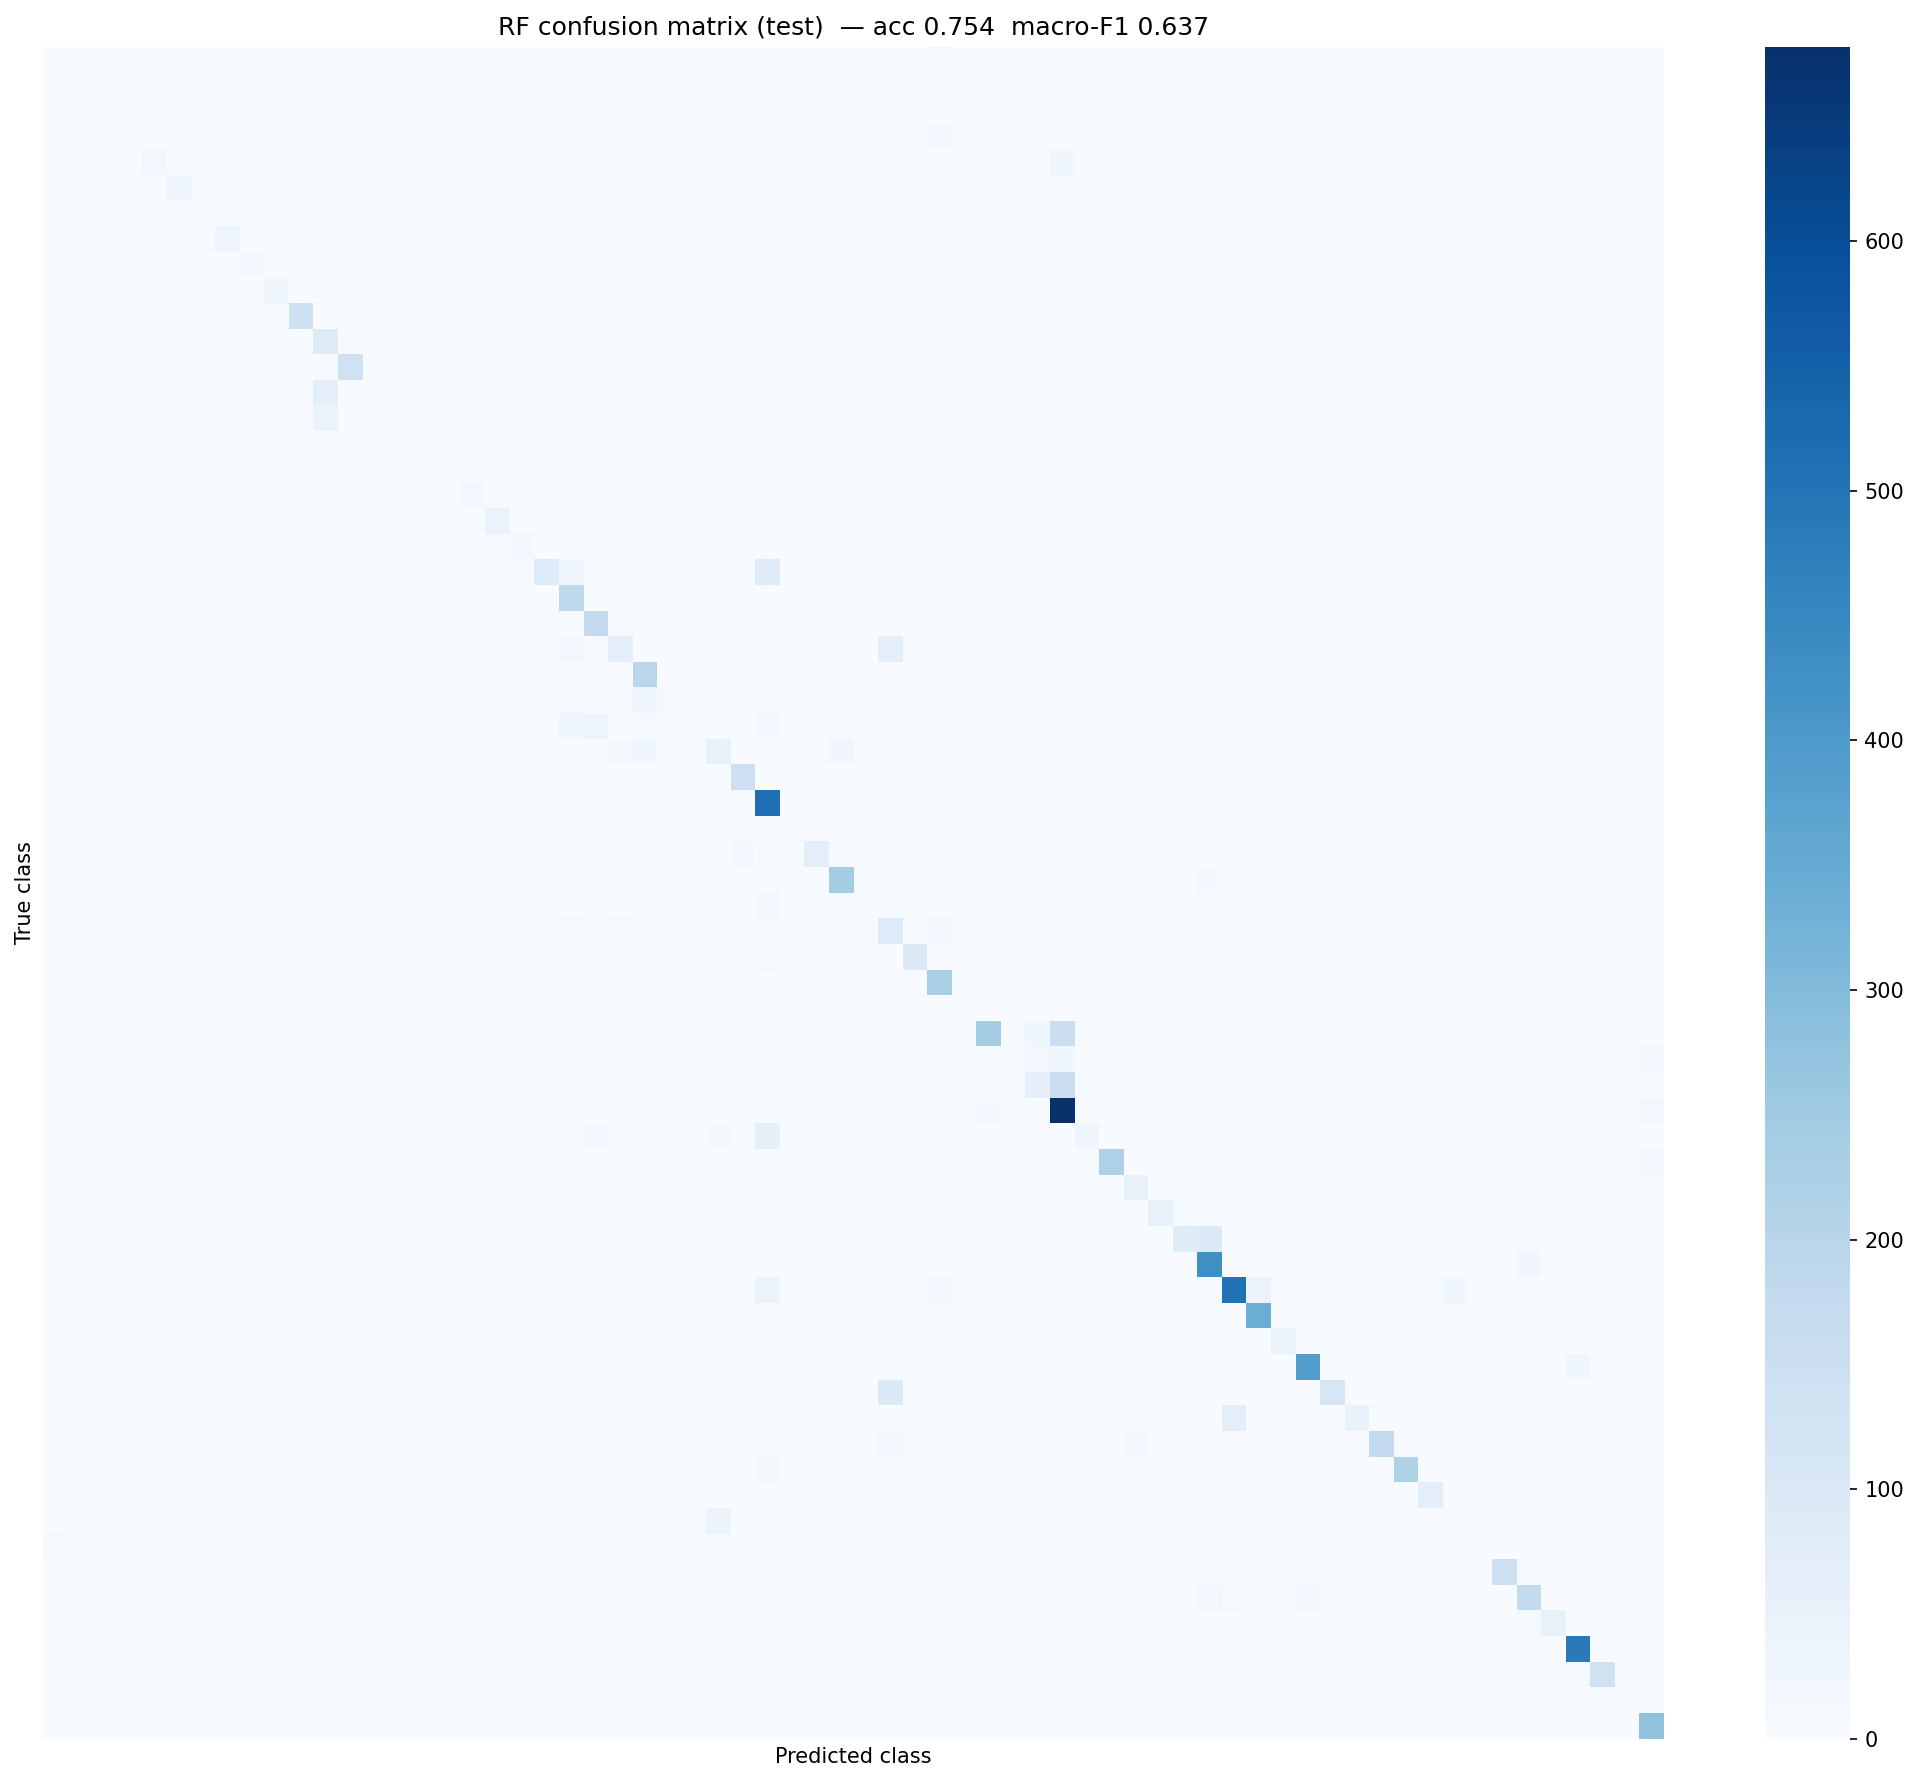
\includegraphics[width=\columnwidth]{images/confusion_matrix_rf.png}
    \caption{Random Forest confusion matrix on the test set (66 classes). Accuracy: 75.4\%, macro-F1: 0.64.}
    \label{fig:cm_rf}
\end{figure}

\section{Model Interpretability}\label{sec:interpretability}

Random Forest provides Gini feature importance scores that indicate which MFCC statistics contribute most to classification.
Figure~\ref{fig:importance} shows the top 20 features.
The most important features are low-order MFCC means (coefficients 0--7), which capture the coarse spectral envelope of insect calls.
Delta coefficients (\texttt{delta1\_std}, \texttt{delta2\_std}) also appear in the top 20, indicating that temporal dynamics contribute to species discrimination.

This analysis is not possible with the CNN baseline, which operates on raw spectrogram images without explicit feature-level attribution.
The RF model thus provides an interpretable complement to the deep learning approach.

\begin{figure}[!t]
    \centering
    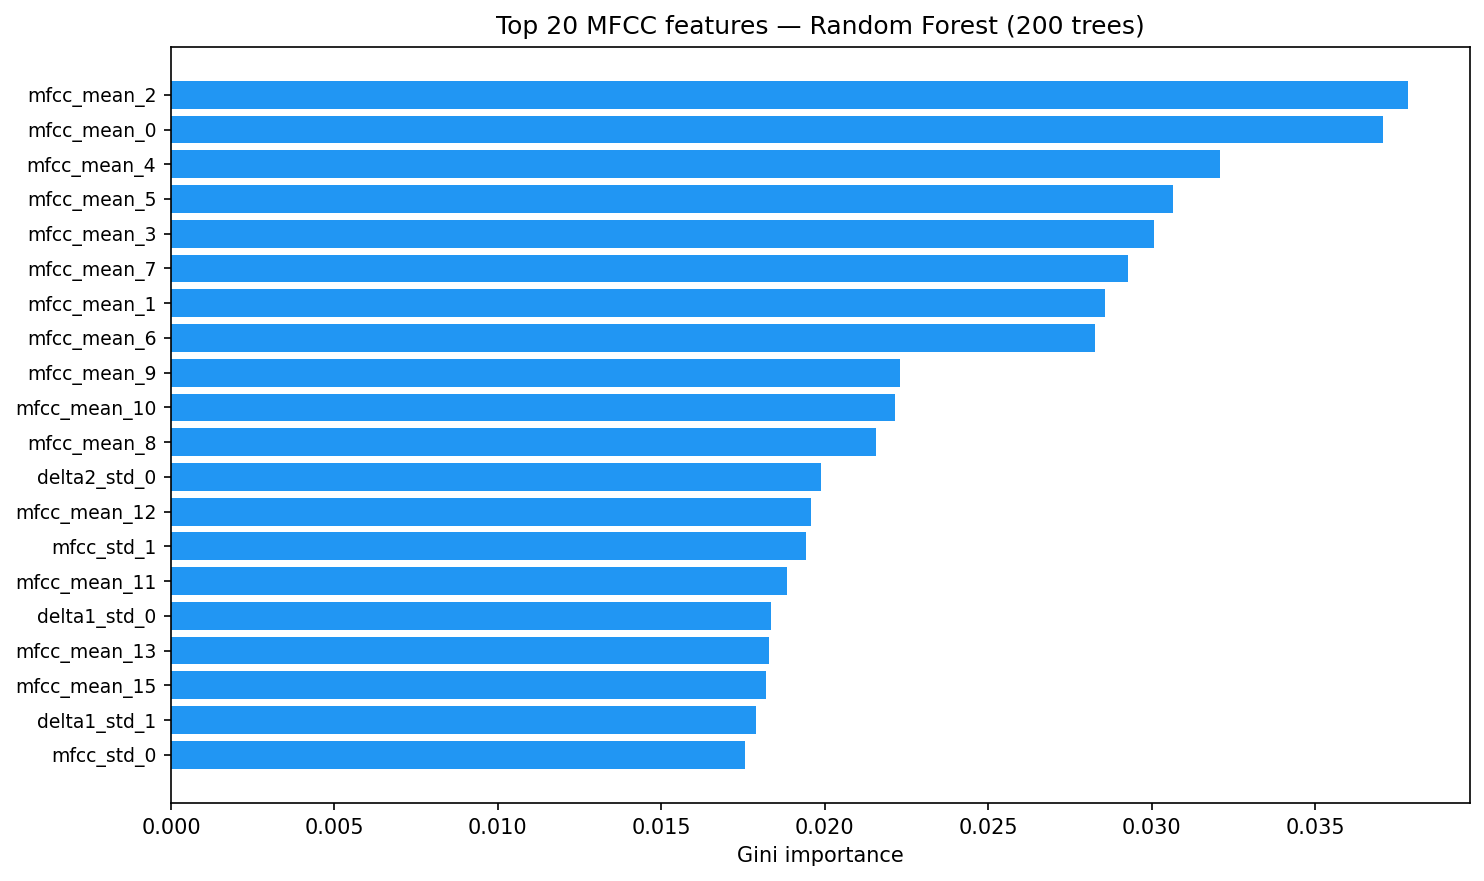
\includegraphics[width=\columnwidth]{images/rf_feature_importance.png}
    \caption{Top 20 MFCC features by Gini importance (Random Forest, 200 trees). Low-order MFCC means dominate, reflecting their importance for encoding spectral shape.}
    \label{fig:importance}
\end{figure}
